\providecommand{\econtexRoot}{.}
% The \commands below are required to allow sharing of the same base code via Github between TeXLive on a local machine and ShareLaTeX.  This is an ugly solution to the requirement that custom LaTeX packages be accessible, and that ShareLaTeX seems to ignore symbolic links (even if they are relative links to valid locations)
\newcommand{\econtex}{\econtexRoot/texmf-local/tex/latex/econtex}
\newcommand{\econtexSetup}{\econtexRoot/texmf-local/tex/latex/econtexSetup}
\newcommand{\econtexShortcuts}{\econtexRoot/texmf-local/tex/latex/econtexShortcuts}
\newcommand{\econtexBibMake}{\econtexRoot/texmf-local/tex/latex/econtexBibMake}
\newcommand{\econtexBibStyle}{\econtexRoot/texmf-local/bibtex/bst/econtex}
\providecommand{\EqDir}{\econtexRoot/Equations}
\providecommand{\FigDir}{\econtexRoot/Figures}
\providecommand{\CodeDir}{\econtexRoot/Code}
\providecommand{\CodeDir}{\econtexRoot/Data}
\providecommand{\SlideDir}{\econtexRoot/Slides}
\providecommand{\TableDir}{\econtexRoot/Tables}
\providecommand{\ResourcesDir}{\econtexRoot/Resources}
%\providecommand{\ApndxDir}{.} % Appendices can be in a subdirectory (and this can be redefined to, say, \providecommand{\ApndxDir}{\econtexRoot/Appendices} only if they do not reference any resources (Tables, Equations, Code, etc) in any other directory

  
\documentclass[titlepage,letterpaper]{\econtex}

\providecommand{\texname}{FaultyPaper}
\usepackage{vmargin}
\usepackage{\econtexSetup}\usepackage{\econtexShortcuts}

\usepackage[en-US]{datetime2}\DTMlangsetup{showdayofmonth=true} 

\provideboolean{ifWeb}\setboolean{ifWeb}{false}\opt{Web}{\setboolean{ifWeb}{true}}

\ifthenelse{\boolean{ifWeb}}{\usepackage{grfext} 
  \PrependGraphicsExtensions*{.svg,.jpg,.JPG,.png,.PNG,.pdf,.PDF}
}{} 

\providecommand{\versn}{} 
\ifthenelse{\boolean{ifWeb}}{  \renewcommand{\ushort}{\underline}\renewcommand{\versn}{Web} }{} 

\newboolean{verbatimwriteOn}   

\setboolean{verbatimwriteOn}{false} 
\newcommand{\ifVerbatimWrite}{\ifthenelse{\boolean{verbatimwriteOn}}} 
\ifVerbatimWrite{}{
  \renewenvironment{verbatimwrite}[1]{} 
} 

\newenvironment{Private}{} 

\providecommand{\wAlt}{\omega}
\providecommand{\sConst}{\varsigma}

\newtheorem{defn}{Definition}
\newtheorem{theorem}{Theorem}
\newtheorem{lemma}{Lemma}
\newtheorem{corollary}{Corollary}
\newtheorem{prop}{Proposition}

\renewcommand{\cite}{\citeyear}

\setmarginsrb{1in}{1in}{1in}{1.4in}{0pt}{0pt}{0pt}{.3in} 

\provideboolean{bigdouble}    
\setboolean{bigdouble}{true} 
\setboolean{bigdouble}{false} 

\ifthenelse{\boolean{bigdouble}}{ 
  \setmarginsrb{0.40in}{0.8in}{0.40in}{0.8in}{0pt}{0pt}{0pt}{0.2in} 
}{} 

\begin{document}\bibliographystyle{\econtexBibStyle}

\hfill{\tiny \texname~\versn~\today~{at} \DTMcurrenttime, \input{.git-source-commit}~~\input{.git-public-commit}}

\title{An Attempt at the Replication of \\ Yongsung Chang and Sun Bin-Kim's \\ Heterogeneity and Aggregation: \\ Implications for Labor-Market Fluctuations}

\newlength\TableWidth

\ifthenelse{\boolean{ifWeb}}{
  \author{
   Wonsik Ko \authNum
    \and
    Syareza Tobing \authNum
  }
}{
  \author{
   Wonsik Ko\authNum \\ {\small Johns Hopkins University}
    \and
   Syareza Tobing\authNum \\ {\small Johns Hopkins University} 
  }
} 

\date{December 22, 2020}
\maketitle

\jelclass{D31, E32, J22, J24, J31\\
  \href{https://econ-ark.org}{
\includegraphics{./Resources/PoweredByEconARK}} \\ \phantom{.}}

\keywords{optimal consumption and labor, heterogeneous-agents, incomplete capital markets, indivisible labor}


\hypertarget{Abstract}{}
\begin{abstract}
This paper adresses the low correlation between hours and productivity in the business cycle literature along with the large cyclical movement in the wedge derived for the intratemporal choice of commodity consumption and hours worked in the business cycle literature. Using only a technology shock as the aggregate disturbance, the authors obtained a low correlation between hours worked and productivity. The interaction between incomplete capital markets and indivisible labor breaks the link between employment and wages at the aggregate level. Aggregate employment is not highly correlated with productivity because individual optimality conditions do not aggregate well.
\end{abstract}

\vspace{-1cm}
\begin{authorsinfo}
  \name{Ko: Department of Economics, Johns Hopkins University, email: \href{mailto:wko5@jhu.edu}{\texttt{wko5@jhu.edu}}}
  \name{Tobing: Department of Economics, Johns Hopkins University, email:  \href{mailto:mtobing1@jhu.edu}{\texttt{mtobing1@jhu.edu}}}
\end{authorsinfo}

\hypertarget{links}{}
\medskip
\begin{small}
  \parbox{\textwidth}{
    \begin{center}
      \begin{tabbing}
        \texttt{Original Papper:~} \= \= \texttt{\href{https://www.aeaweb.org/articles?id=10.1257/aer.97.5.1939}{American Economic Association (Paywall)}} \\
        \texttt{~~~GitHub:~} \> \> \texttt{\href{https://github.com/raytobing/final_project/tree/master/replication}{Replication Project}} \\
      \end{tabbing}
    \end{center}

  } 
\end{small}

\titlepagefinish

\setcounter{page}{1}

\setcounter{footnote}{0}

\ifthenelse{\boolean{ifWeb}}{\thankstext}{}

\hypertarget{Introduction}{}
\section{Introduction}\label{sec:Intro}

\begin{verbatimwrite}{./Sections/Intro.tex} 

  \citet{changkim2007} is a broken paper with an aesthetic in code writing reminiscent of Korean art (no, that's not a compliment). Basically, we really just want to replicate Figure \ref{fig:goal} shown below, specifically the third line as written in the legend box. While we understand that an honest replication should aim for the first line, we have realized that that particular line is beyond our current capabilities to reproduce at this moment at given the time. So there you go. We will show you what we managed in these few grueling months.

  \begin{figure}[ht]
    {\centering \includegraphics[width=.95\textwidth]{\FigDir/figure_5.pdf}}
    \caption{Labor-Market Wedges From The Models}
    \footnotesize {{\emph{Source:}} {\citet{changkim2007}}}
    \label{fig:goal}
  \end{figure}

  $$U(C_t , H_t) \ = \ lnC_t \ - \ B \bigg[ \frac{H^{1+1/\gamma}}{(1 \ + \frac{1}{\gamma})} \bigg]$$

\begin{align*}
C_t \    &: \text{commodity consumption}\\
H_t \    &: \text{hours worked}\\
\gamma \ &: \text{compensated labor supply elasticity}\\
B \      &: \text{constant}
\end{align*}
  
 Assuming an aggregate Cobb-Douglas production function with labor-income share denoted by $\alpha$, the Marginal Rate of Stubstitution (MRS) should be equal to the Marginal Productivity of Labor (MPL):

 $$B \frac{H_t^{1/\gamma}}{C_t^{-1}} \ = \ \alpha \frac{Y_t}{H_t}$$

 Nevertheless, as we can see from Figure \ref{fig:figure_1}, the MRS is more volatile that hours and often moves in opposite direction to productivity, thereby violating the equilibrium.

     \begin{figure}[ht]
    {\centering \includegraphics[width=.95\textwidth]{\FigDir/figure_1.pdf}}
    \caption{Cyclical Components of MRS and Labor Productivity}
    \footnotesize {{\emph{Source:}} {\citet{changkim2007}}}
    \label{fig:figure_1}
  \end{figure}

On the other hand, the labor-market wedge is defines as:
$$ln \ Wedge_t \ = \ ln \ MRS_t \ - \ ln\frac{Y_t}{H_t} \ + \ constant$$

Figure 2 shows that the wedge is highly correlated with hours worked and its volatility has similar magnitude as hours worked. The wedge arises because hours worked are not highly correlated with productivity.

     \begin{figure}[ht]
    {\centering \includegraphics[width=.95\textwidth]{\FigDir/figure_2.pdf}}
    \caption{Cyclical Components of Hours and Labor-Market Wedge for The United States}
    \footnotesize {{\emph{Source:}} {\citet{changkim2007}}}
    \label{fig:figure_2}
  \end{figure}


\end{verbatimwrite}\ifVerbatimWrite{\input{Sections/Intro}}{}

\hypertarget{Model}{}
\section{The Model}\label{sec:Model}

\begin{verbatimwrite}{./Sections/Setup-Intro}

\subsection{Setup}\label{sec:Setup}  

The model is an extension of Krussel-Smith's (1998) heterogeneous agent model with incomplete capital markets to indivisible labor supply. A continuum of workers have identical preferences but different productivity along with a separable preference over consumption and hours worked. Capital markets are incomplete. Workers trade claims for physical capital, $a_t$ that yields a return of $r_t$ Workers face a borrowing constraint $a_t \geq \bar{a},$ for all t. Labor supply is indivisible such that if employed, a worker supplies $\bar{h}$ units of labor and earns $w_t x_t \bar{h}$ where:
\begin{itemize}
    \item $w_t$: wage rate per effective unit of labor
    \item $x_t$: individual productivity
    \end{itemize}

   $w_t$ varies exogenously according to a stochastic process with a transition probability distribution function defined as:
    \begin{itemize}
    \item $\pi_x(x'|x) \ = \ Pr(x_{t+1} \leq \ x'|x_t \ = \ x)$
    \item $x_t$ is the only idiosyncratic risk faced by the agents in the model and the only source of heterogeneity
    \end{itemize}

    Output is produced through a Cobb-Douglas Production function defined by:
    $Y_t \ = \ F(L_t,K_t, \lambda_t) \ = \ \lambda_t L^\alpha_t K^{1-\alpha}_t$
    \begin{itemize}
        \item $K_t$: capital which depreciates at rate $\delta$ each period
       \item $L_t$: effective units of labor
       \item $\mu$: distribution of workers
       \item $\lambda$: aggregate productivity 
       \end{itemize}

      $\lambda$ evolves with a transition probability distribution function:
           $$\pi_\lambda (\lambda'|\lambda) \ = \ Pr(\lambda_{t+1} \leq \lambda ' | \lambda_t \ = \ \lambda)$$

     The value function for an employed worker is:

     \begin{align*}
      \begin{split}
 V^E (a,& \ x; \ \lambda, \ \mu)\\
 = & \max_{a' \ \in \ A} \bigg\{ ln \ c \ - \ B \frac{h^{1 \ 1/ \gamma}}{1 \ + \ 1/ \gamma}\\
 \\
 & + \ \beta E[max \{ V^E (a',x';\lambda ', \mu'), \ V^N (a',x'; \lambda ', \mu ') \}|x, \lambda] \bigg\},\\
\end{split}
     \end{align*}

     subject to:

 $$c \ = \ w( \lambda, \mu )x \bar{h} \ + \ (1 \ + \ r)\lambda,\mu))a \ - \ a',$$
 $$a' \geq \bar{a},$$
 $$\mu ' \ = \mathbb{T}(\lambda,\mu)$$

        where $\mathbb{T}$ is a transition operator defining the law of motion for the distribution of worker $\mu$. The value function of non-employed worker (h = 0) is defined by:
$$V(a,x; \lambda,\mu) \ = \max_{h \in \{0, \bar{h}\}} \{V^E (a,x; \lambda, \mu), \ V^N (a,x;\lambda,\mu) \}$$

\subsection{Equilibrium Conditions}\label{sec:Equilibrium}

Equilibrium consists of:
\begin{enumerate}
  \item A set of value functions
    \begin{itemize}
    \item $ V^E (a,x;\lambda,\mu), \ V^N (a,x;\lambda,\mu), \  V (a,x;\lambda,\mu)$
    \end{itemize}
  \item A set of decision rules for consumption, asset holdings and labor supply
     \begin{itemize}
    \item $\{c(a,x;\lambda,\mu), \ a'(a,x;\lambda,\mu), \ h(a,x;\lambda,\mu)\}$
    \end{itemize}
  \item A set of decision rules for aggregate inputs
     \begin{itemize}
    \item  $\{K (\lambda,\mu),L(\lambda,\mu)\}$
    \end{itemize}
  \item A set of decision rules for factor prices
     \begin{itemize}
    \item $\{ w(\lambda,\mu),r(\lambda,\mu)\}$
    \end{itemize}
  \item Law of motion for the distribution of workers
     \begin{itemize}
    \item $\mu ' \ = \ \mathbb{T}(\lambda,\mu)$
    \end{itemize}
  \end{enumerate}

  such that:
  
  \begin{enumerate}
    
\item Individuals optimizes given $w(\lambda,\mu)$ and $r(\lambda,\mu)$.

\item Representative firms maximizing profits.
$$w(\lambda,\mu) \ = \ F_1 (L(\lambda,\mu), K(\lambda,\mu), \lambda)$$
$$r(\lambda,\mu) \ = \ F_2 (L(\lambda,\mu), K(\lambda,\mu), \lambda) \ - \ \delta$$

\item The goods market clears.
$$\int \{ a'(a,x; \lambda, \mu) \ + \ c(a,x; \lambda, \mu)\} d \mu $$
$$= \ F(L(\lambda,\mu), K(\lambda,\mu), \lambda) \ + \ (1 \ - \ \delta)$$

\item Factor market clears.
$$L(\lambda,\mu) \ = \ \int xh(a,x;\lambda,\mu) \ d \mu$$
$$K(\lambda,\mu) \ = \ \int a \ d \mu$$

\item Individual and aggregate behaviours are consistent.
$$\mu ' (A^0 , \ X^0)$$
$$ = \int_{A^0 , X^0} \int_{A,\chi} \mathbbm{1}_{a'=a'(a,x;\lambda,\mu)} d\pi_x (x'|x)d\mu \} da'dx'$$

\end{enumerate}
  
\end{verbatimwrite}\ifVerbatimWrite{\input{Sections/Model}}{}

\section{Quantitative Analysis}\label{sec:QuantAnalysis}

\subsection{Calibration}\label{sec:Calibration}

The unit of time is business quarter and parameters are obtained from the Panel Study of Income Dynamics (PSID) along with the empirical labor supply literature. Parameters are summarized in Table \ref{fig:table_1} below:

     \begin{figure}[ht]
    {\centering \includegraphics[width=.95\textwidth]{\FigDir/table_1.pdf}}
    \caption{Parameters of the Benchmark Model Economy}
    \footnotesize {{\emph{Source:}} {\citet{changkim2007}}}
    \label{fig:table_1}
  \end{figure}

  \subsection{Cross-Sectinal Distribution for Earnings, Wealth and Reservation Wages}\label{sec:CrossSectional}

       \begin{figure}[ht]
    {\centering \includegraphics[width=.95\textwidth]{\FigDir/table_2.pdf}}
    \caption{Characteristics of Wealth Distribution}
    \footnotesize {{\emph{Source:}} {\citet{changkim2007}}}
    \label{fig:table_2}
  \end{figure}
  
Table \ref{fig:table_2}  summarizes the PSID and the model's information on wealth and earnings. For each quintile group of wealth distribution, the authors calculated:

\begin{enumerate}
\item Wealth share
\item ratio of group average to economy-wide average
\item Earnings share
\end{enumerate}

In the model, labor-market participation is determined by market opportunity (wage) and wealth (asset holdings). The steady-state reservation wage schedule is shown in Figure \ref{fig:figure_3}  below.

     \begin{figure}[ht]
    {\centering \includegraphics[width=.95\textwidth]{\FigDir/figure_3.pdf}}
    \caption{Reservation Wages From the Benchmark Model}
    \footnotesize {{\emph{Source:}} {\citet{changkim2007}}}
    \label{fig:figure_3}
  \end{figure}


\subsection{Cyclical Properties of the Model}\label{sec:CyclicalProperties}

The equilibrium of the model is solved using the "bounded rationality" method developed by Krussel Smith (1998) where agents uses a finite set of moments of $\mu$ in forecasting aggregate prices. Table \ref{fig:table_3}  below presents the volatility of key aggregate variables in the model economy.

       \begin{figure}[ht]
    {\centering \includegraphics[width=.95\textwidth]{\FigDir/table_3.pdf}}
    \caption{Volatilities of Aggregate Variables}
    \footnotesize {{\emph{Source:}} {\citet{changkim2007}}}
    \label{fig:table_3}
  \end{figure}
  

These main observations obtained from Table 3 are:
\begin{itemize}
\item Ouput volatility is less than 2/3 of actual output volatility, similar to that of the standard representative agent models.
\item Volatility of hours relative to output and the volatility of labor productivity relative to output is the same as that in the data
\item The realtive volatility of hours to productivity is very colse to that in the data.
\end{itemize}

Table \ref{fig:table_4}  below shows the cyclicality of key aggregate variables.

       \begin{figure}[ht]
    {\centering \includegraphics[width=.95\textwidth]{\FigDir/table_4.pdf}}
    \caption{Cyclicality of Aggregate Variables}
    \footnotesize {{\emph{Source:}} {\citet{changkim2007}}}
    \label{fig:table_4}
  \end{figure}
  
The main observations obtained from Table \ref{fig:table_4}  are:
\begin{itemize}
\item The correlation between output, consumption, investment and labor productivity are higher than the data, a common feature of standard RBC models.
\item The correlation of hours with output is close to the data
\item Hours worked and labor productivity has low correlation despite aggregate productivity shock being the sole driving force in the simulation.
  \end{itemize} 

\hypertarget{LCandCCIntro}{}

\section{Conclusion}

The fact that hours worked are not strongly correlated with labor productivity has been considered as a shortcoming of equilibrium business cycle theory. Using a heterogeneous-agent economy with incomplete capital markets and indivisible labor, the authors show that they can generate a low employment-productivity correlation. When the optimality condition implied by the representative agent is applied to the model, the authors were also able to find a time-varying wedge between MRS and MPL without the addition of distortion nor exogenous labor-supply shock.

\vfill\eject
\appendix

\centerline{\LARGE Appendix}
\medskip

\hfill

The replication of this paper utilizes the Econ-ARK/HARK toolkit to attempt at a reproduction of a figure produced in the original paper, specifically Figure 5. In order to do so, the main HARK tool used here is $\texttt{ConsAggShockModel}$ and $\texttt{ConsLaborModel}$ class, portions of which we've combined to create a new class named $\texttt{ConsLaborAggMarkov}$ in which agents have the utility function described in the main body of the paper and face idiosyncratic shocks their productivity.

  \begin{figure}[ht]
    {\centering 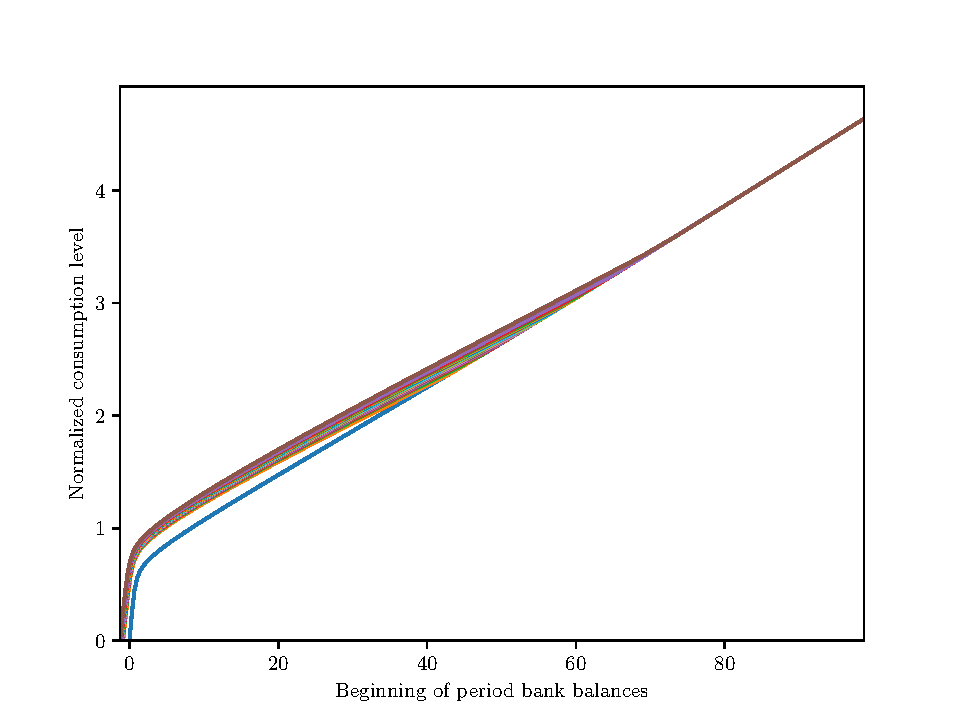
\includegraphics[width=.95\textwidth]{\FigDir/conslabor1.pdf}}
    \caption{Placemat of what is produced by a Python Code}
    \footnotesize {\emph{Source: Econ-Ark}}
    \label{fig:codeproduced}
  \end{figure}

Given the current limitations of the $\texttt{ConsLaborModel}$, we were not able to incorporate the artificial borrowing constraint into the final replication model. 

\clearpage\pagebreak\vfill\eject

\bibliography{LiqConstr,LiqConstr-Add,economics}\end{document}
